% Options for packages loaded elsewhere
\PassOptionsToPackage{unicode}{hyperref}
\PassOptionsToPackage{hyphens}{url}
\PassOptionsToPackage{dvipsnames,svgnames,x11names}{xcolor}
%
\documentclass[
  letterpaper,
  DIV=11,
  numbers=noendperiod]{scrartcl}

\usepackage{amsmath,amssymb}
\usepackage{iftex}
\ifPDFTeX
  \usepackage[T1]{fontenc}
  \usepackage[utf8]{inputenc}
  \usepackage{textcomp} % provide euro and other symbols
\else % if luatex or xetex
  \usepackage{unicode-math}
  \defaultfontfeatures{Scale=MatchLowercase}
  \defaultfontfeatures[\rmfamily]{Ligatures=TeX,Scale=1}
\fi
\usepackage{lmodern}
\ifPDFTeX\else  
    % xetex/luatex font selection
\fi
% Use upquote if available, for straight quotes in verbatim environments
\IfFileExists{upquote.sty}{\usepackage{upquote}}{}
\IfFileExists{microtype.sty}{% use microtype if available
  \usepackage[]{microtype}
  \UseMicrotypeSet[protrusion]{basicmath} % disable protrusion for tt fonts
}{}
\makeatletter
\@ifundefined{KOMAClassName}{% if non-KOMA class
  \IfFileExists{parskip.sty}{%
    \usepackage{parskip}
  }{% else
    \setlength{\parindent}{0pt}
    \setlength{\parskip}{6pt plus 2pt minus 1pt}}
}{% if KOMA class
  \KOMAoptions{parskip=half}}
\makeatother
\usepackage{xcolor}
\setlength{\emergencystretch}{3em} % prevent overfull lines
\setcounter{secnumdepth}{-\maxdimen} % remove section numbering
% Make \paragraph and \subparagraph free-standing
\makeatletter
\ifx\paragraph\undefined\else
  \let\oldparagraph\paragraph
  \renewcommand{\paragraph}{
    \@ifstar
      \xxxParagraphStar
      \xxxParagraphNoStar
  }
  \newcommand{\xxxParagraphStar}[1]{\oldparagraph*{#1}\mbox{}}
  \newcommand{\xxxParagraphNoStar}[1]{\oldparagraph{#1}\mbox{}}
\fi
\ifx\subparagraph\undefined\else
  \let\oldsubparagraph\subparagraph
  \renewcommand{\subparagraph}{
    \@ifstar
      \xxxSubParagraphStar
      \xxxSubParagraphNoStar
  }
  \newcommand{\xxxSubParagraphStar}[1]{\oldsubparagraph*{#1}\mbox{}}
  \newcommand{\xxxSubParagraphNoStar}[1]{\oldsubparagraph{#1}\mbox{}}
\fi
\makeatother


\providecommand{\tightlist}{%
  \setlength{\itemsep}{0pt}\setlength{\parskip}{0pt}}\usepackage{longtable,booktabs,array}
\usepackage{calc} % for calculating minipage widths
% Correct order of tables after \paragraph or \subparagraph
\usepackage{etoolbox}
\makeatletter
\patchcmd\longtable{\par}{\if@noskipsec\mbox{}\fi\par}{}{}
\makeatother
% Allow footnotes in longtable head/foot
\IfFileExists{footnotehyper.sty}{\usepackage{footnotehyper}}{\usepackage{footnote}}
\makesavenoteenv{longtable}
\usepackage{graphicx}
\makeatletter
\newsavebox\pandoc@box
\newcommand*\pandocbounded[1]{% scales image to fit in text height/width
  \sbox\pandoc@box{#1}%
  \Gscale@div\@tempa{\textheight}{\dimexpr\ht\pandoc@box+\dp\pandoc@box\relax}%
  \Gscale@div\@tempb{\linewidth}{\wd\pandoc@box}%
  \ifdim\@tempb\p@<\@tempa\p@\let\@tempa\@tempb\fi% select the smaller of both
  \ifdim\@tempa\p@<\p@\scalebox{\@tempa}{\usebox\pandoc@box}%
  \else\usebox{\pandoc@box}%
  \fi%
}
% Set default figure placement to htbp
\def\fps@figure{htbp}
\makeatother
% definitions for citeproc citations
\NewDocumentCommand\citeproctext{}{}
\NewDocumentCommand\citeproc{mm}{%
  \begingroup\def\citeproctext{#2}\cite{#1}\endgroup}
\makeatletter
 % allow citations to break across lines
 \let\@cite@ofmt\@firstofone
 % avoid brackets around text for \cite:
 \def\@biblabel#1{}
 \def\@cite#1#2{{#1\if@tempswa , #2\fi}}
\makeatother
\newlength{\cslhangindent}
\setlength{\cslhangindent}{1.5em}
\newlength{\csllabelwidth}
\setlength{\csllabelwidth}{3em}
\newenvironment{CSLReferences}[2] % #1 hanging-indent, #2 entry-spacing
 {\begin{list}{}{%
  \setlength{\itemindent}{0pt}
  \setlength{\leftmargin}{0pt}
  \setlength{\parsep}{0pt}
  % turn on hanging indent if param 1 is 1
  \ifodd #1
   \setlength{\leftmargin}{\cslhangindent}
   \setlength{\itemindent}{-1\cslhangindent}
  \fi
  % set entry spacing
  \setlength{\itemsep}{#2\baselineskip}}}
 {\end{list}}
\usepackage{calc}
\newcommand{\CSLBlock}[1]{\hfill\break\parbox[t]{\linewidth}{\strut\ignorespaces#1\strut}}
\newcommand{\CSLLeftMargin}[1]{\parbox[t]{\csllabelwidth}{\strut#1\strut}}
\newcommand{\CSLRightInline}[1]{\parbox[t]{\linewidth - \csllabelwidth}{\strut#1\strut}}
\newcommand{\CSLIndent}[1]{\hspace{\cslhangindent}#1}

\KOMAoption{captions}{tableheading}
\makeatletter
\@ifpackageloaded{caption}{}{\usepackage{caption}}
\AtBeginDocument{%
\ifdefined\contentsname
  \renewcommand*\contentsname{Table of contents}
\else
  \newcommand\contentsname{Table of contents}
\fi
\ifdefined\listfigurename
  \renewcommand*\listfigurename{List of Figures}
\else
  \newcommand\listfigurename{List of Figures}
\fi
\ifdefined\listtablename
  \renewcommand*\listtablename{List of Tables}
\else
  \newcommand\listtablename{List of Tables}
\fi
\ifdefined\figurename
  \renewcommand*\figurename{Figure}
\else
  \newcommand\figurename{Figure}
\fi
\ifdefined\tablename
  \renewcommand*\tablename{Table}
\else
  \newcommand\tablename{Table}
\fi
}
\@ifpackageloaded{float}{}{\usepackage{float}}
\floatstyle{ruled}
\@ifundefined{c@chapter}{\newfloat{codelisting}{h}{lop}}{\newfloat{codelisting}{h}{lop}[chapter]}
\floatname{codelisting}{Listing}
\newcommand*\listoflistings{\listof{codelisting}{List of Listings}}
\makeatother
\makeatletter
\makeatother
\makeatletter
\@ifpackageloaded{caption}{}{\usepackage{caption}}
\@ifpackageloaded{subcaption}{}{\usepackage{subcaption}}
\makeatother

\usepackage{bookmark}

\IfFileExists{xurl.sty}{\usepackage{xurl}}{} % add URL line breaks if available
\urlstyle{same} % disable monospaced font for URLs
\hypersetup{
  pdftitle={Neuroanatomy},
  colorlinks=true,
  linkcolor={blue},
  filecolor={Maroon},
  citecolor={Blue},
  urlcolor={Blue},
  pdfcreator={LaTeX via pandoc}}


\title{Neuroanatomy}
\usepackage{etoolbox}
\makeatletter
\providecommand{\subtitle}[1]{% add subtitle to \maketitle
  \apptocmd{\@title}{\par {\large #1 \par}}{}{}
}
\makeatother
\subtitle{PSY 511.003 Spr 2025}
\author{}
\date{}

\begin{document}
\maketitle


\section{Prelude}\label{prelude}

\begin{center}\rule{0.5\linewidth}{0.5pt}\end{center}

\begin{center}\rule{0.5\linewidth}{0.5pt}\end{center}

\subsection{Announcements}\label{announcements}

\begin{itemize}
\tightlist
\item
  Exercise 02 {due next Wednesday, January 29, 2025}.
\end{itemize}

\subsection{Today's topics}\label{todays-topics}

\begin{itemize}
\tightlist
\item
  Neuroanatomy

  \begin{itemize}
  \tightlist
  \item
    Brief overview
  \item
    In-class lab
  \item
    \href{../exercises/ex02.qmd}{Exercise 02}
  \end{itemize}
\end{itemize}

\section{Neuroanatomy}\label{neuroanatomy}

\subsection{Why study?}\label{why-study}

\begin{itemize}
\tightlist
\item
  Master basic vocabulary for reading literature
\end{itemize}

\subsection{Brain anatomy through
dance}\label{brain-anatomy-through-dance}

Your browser does not support the audio tag.

\subsection{Directional terms}\label{directional-terms}

\begin{itemize}
\tightlist
\item
  Anterior/Posterior
\item
  Medial/Lateral
\item
  Superior/Inferior
\item
  Dorsal/Ventral
\item
  Rostral/Caudal
\end{itemize}

\subsection{Central vs.~Peripheral Nervous
System}\label{central-vs.-peripheral-nervous-system}

\begin{figure}[H]

{\centering \pandocbounded{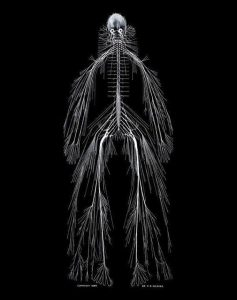
\includegraphics[keepaspectratio]{wk02-2025-01-23_files/mediabag/harriet-bw-237w.jpg}}

}

\caption{Nervous system of Harriet Cole, see McNaughton (2018)}

\end{figure}%

\subsection{Organization of the CNS}\label{organization-of-the-cns}

\begin{longtable}[]{@{}
  >{\raggedright\arraybackslash}p{(\linewidth - 6\tabcolsep) * \real{0.2500}}
  >{\raggedright\arraybackslash}p{(\linewidth - 6\tabcolsep) * \real{0.2500}}
  >{\raggedright\arraybackslash}p{(\linewidth - 6\tabcolsep) * \real{0.2500}}
  >{\raggedright\arraybackslash}p{(\linewidth - 6\tabcolsep) * \real{0.2500}}@{}}
\toprule\noalign{}
\begin{minipage}[b]{\linewidth}\raggedright
Major division
\end{minipage} & \begin{minipage}[b]{\linewidth}\raggedright
Ventricular Landmark
\end{minipage} & \begin{minipage}[b]{\linewidth}\raggedright
Embryonic Division
\end{minipage} & \begin{minipage}[b]{\linewidth}\raggedright
Structure
\end{minipage} \\
\midrule\noalign{}
\endhead
\bottomrule\noalign{}
\endlastfoot
Forebrain & Lateral & Telencephalon & Cerebral cortex \\
& & & Basal ganglia \\
& & & Hippocampus, amygdala \\
\end{longtable}

\begin{center}\rule{0.5\linewidth}{0.5pt}\end{center}

\begin{longtable}[]{@{}
  >{\raggedright\arraybackslash}p{(\linewidth - 6\tabcolsep) * \real{0.2222}}
  >{\raggedright\arraybackslash}p{(\linewidth - 6\tabcolsep) * \real{0.3056}}
  >{\raggedright\arraybackslash}p{(\linewidth - 6\tabcolsep) * \real{0.2778}}
  >{\raggedright\arraybackslash}p{(\linewidth - 6\tabcolsep) * \real{0.1944}}@{}}
\toprule\noalign{}
\begin{minipage}[b]{\linewidth}\raggedright
Major division
\end{minipage} & \begin{minipage}[b]{\linewidth}\raggedright
Ventricular Landmark
\end{minipage} & \begin{minipage}[b]{\linewidth}\raggedright
Embryonic Division
\end{minipage} & \begin{minipage}[b]{\linewidth}\raggedright
Structure
\end{minipage} \\
\midrule\noalign{}
\endhead
\bottomrule\noalign{}
\endlastfoot
& Third & Diencephalon & Thalamus \\
& & & Hypothalamus \\
\end{longtable}

\begin{center}\rule{0.5\linewidth}{0.5pt}\end{center}

\begin{longtable}[]{@{}
  >{\raggedright\arraybackslash}p{(\linewidth - 6\tabcolsep) * \real{0.2078}}
  >{\raggedright\arraybackslash}p{(\linewidth - 6\tabcolsep) * \real{0.2857}}
  >{\raggedright\arraybackslash}p{(\linewidth - 6\tabcolsep) * \real{0.2597}}
  >{\raggedright\arraybackslash}p{(\linewidth - 6\tabcolsep) * \real{0.2468}}@{}}
\toprule\noalign{}
\begin{minipage}[b]{\linewidth}\raggedright
Major division
\end{minipage} & \begin{minipage}[b]{\linewidth}\raggedright
Ventricular Landmark
\end{minipage} & \begin{minipage}[b]{\linewidth}\raggedright
Embryonic Division
\end{minipage} & \begin{minipage}[b]{\linewidth}\raggedright
Structure
\end{minipage} \\
\midrule\noalign{}
\endhead
\bottomrule\noalign{}
\endlastfoot
Midbrain & Cerebral Aqueduct & Mesencephalon & Tectum, tegmentum \\
\end{longtable}

\begin{center}\rule{0.5\linewidth}{0.5pt}\end{center}

\begin{longtable}[]{@{}
  >{\raggedright\arraybackslash}p{(\linewidth - 6\tabcolsep) * \real{0.2078}}
  >{\raggedright\arraybackslash}p{(\linewidth - 6\tabcolsep) * \real{0.2857}}
  >{\raggedright\arraybackslash}p{(\linewidth - 6\tabcolsep) * \real{0.2597}}
  >{\raggedright\arraybackslash}p{(\linewidth - 6\tabcolsep) * \real{0.2468}}@{}}
\toprule\noalign{}
\begin{minipage}[b]{\linewidth}\raggedright
Major division
\end{minipage} & \begin{minipage}[b]{\linewidth}\raggedright
Ventricular Landmark
\end{minipage} & \begin{minipage}[b]{\linewidth}\raggedright
Embryonic Division
\end{minipage} & \begin{minipage}[b]{\linewidth}\raggedright
Structure
\end{minipage} \\
\midrule\noalign{}
\endhead
\bottomrule\noalign{}
\endlastfoot
Hindbrain & 4th & Metencephalon & Cerebellum, pons \\
& -- & Mylencephalon & Medulla oblongata \\
\end{longtable}

\begin{center}\rule{0.5\linewidth}{0.5pt}\end{center}

Forebrain, midbrain, hindbrain terminology derives from embryonic stages
in CNS development.

\begin{figure}[H]

{\centering \pandocbounded{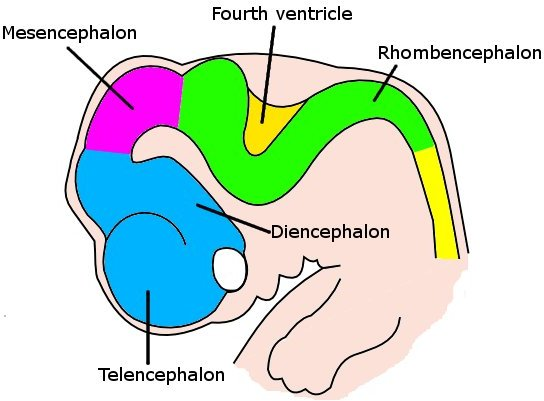
\includegraphics[keepaspectratio]{wk02-2025-01-23_files/mediabag/6_week_embryo_brain.jpg}}

}

\caption{Embryonic human brain from Wikipedia}

\end{figure}%

\subsection{Cerebrum}\label{cerebrum}

\begin{itemize}
\tightlist
\item
  (Cerebral) cortex
\item
  Subcortical (below the cortex) structures
\end{itemize}

\begin{figure}[H]

{\centering \pandocbounded{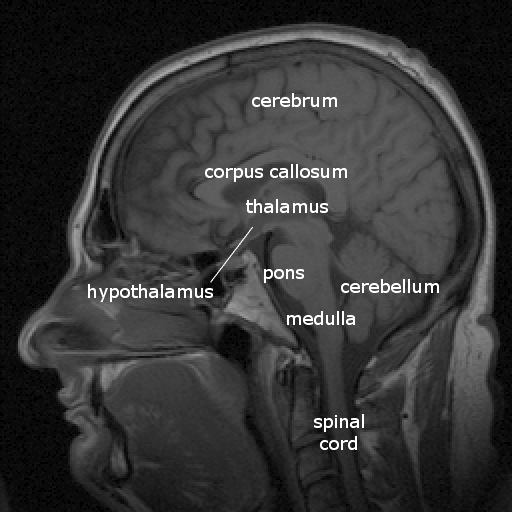
\includegraphics[keepaspectratio]{wk02-2025-01-23_files/mediabag/medial-labelled.gif}}

}

\caption{Labelled MRI including thalamus and hypothalamus}

\end{figure}%

\subsection{(Cerebral) cortex}\label{cerebral-cortex}

\begin{itemize}
\tightlist
\item
  Lobes, marked by sulci/fissures, adjacency to bones of skull
\item
  Functional areas marked by gyri \& sulci
\item
  \href{../resources/anatomy.qmd\#brodmann-areas}{Brodmann Areas}

  \begin{itemize}
  \tightlist
  \item
    Microstructural (cellular composition) features
  \end{itemize}
\end{itemize}

\begin{center}\rule{0.5\linewidth}{0.5pt}\end{center}

\begin{itemize}
\tightlist
\item
  Most lobes host primary sensory or motor area

  \begin{itemize}
  \tightlist
  \item
    Frontal: Motor cortex
  \item
    Temporal: Auditory cortex
  \item
    Parietal: Somatosensory cortex
  \item
    Occipital: Visual cortex
  \item
    Insula: Gustatory
  \end{itemize}
\end{itemize}

\subsection{Input/output}\label{inputoutput}

\begin{itemize}
\tightlist
\item
  Via cranial nerves (in CNS)
\item
  Via spinal nerves (in PNS)
\end{itemize}

\begin{center}\rule{0.5\linewidth}{0.5pt}\end{center}

\begin{figure}[H]

{\centering \pandocbounded{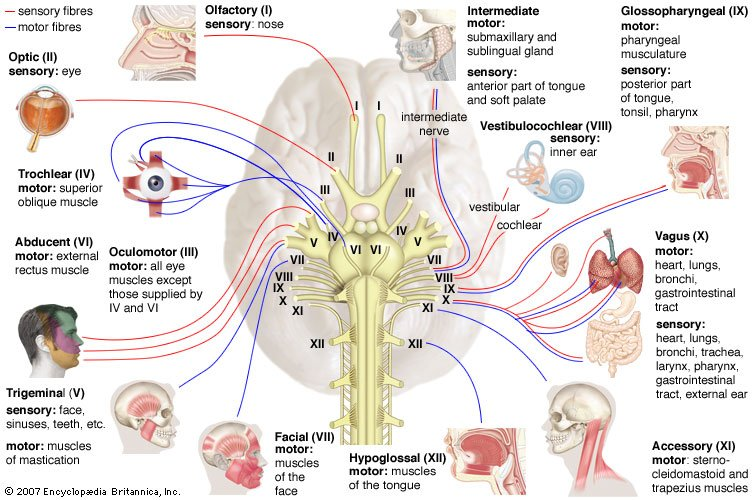
\includegraphics[keepaspectratio]{wk02-2025-01-23_files/mediabag/nerves-pairs-muscles.jpg}}

}

\caption{Cranial nerves from
https://www.britannica.com/science/cranial-nerve\#/media/1/141797/46720}

\end{figure}%

\begin{center}\rule{0.5\linewidth}{0.5pt}\end{center}

\pandocbounded{\includegraphics[keepaspectratio]{wk02-2025-01-23_files/mediabag/Diagram-showing-the-.jpg}}

\begin{center}\rule{0.5\linewidth}{0.5pt}\end{center}

Multiple hierarchies

\begin{figure}[H]

{\centering \pandocbounded{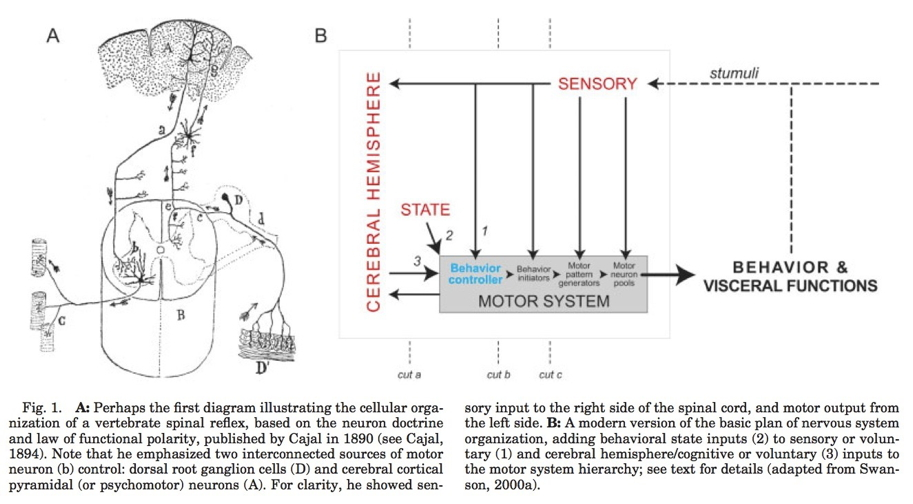
\includegraphics[keepaspectratio]{../include/img/swanson-2005-fig-1.jpg}}

}

\caption{(Swanson, 2005, fig. 1)}

\end{figure}%

\subsection{Maps}\label{maps}

\begin{itemize}
\tightlist
\item
  Sensory \& motor systems often use maps
\end{itemize}

\begin{center}\rule{0.5\linewidth}{0.5pt}\end{center}

\pandocbounded{\includegraphics[keepaspectratio]{wk02-2025-01-23_files/mediabag/The-Retinotopy-parad.png}}

\begin{center}\rule{0.5\linewidth}{0.5pt}\end{center}

\begin{figure}[H]

{\centering \pandocbounded{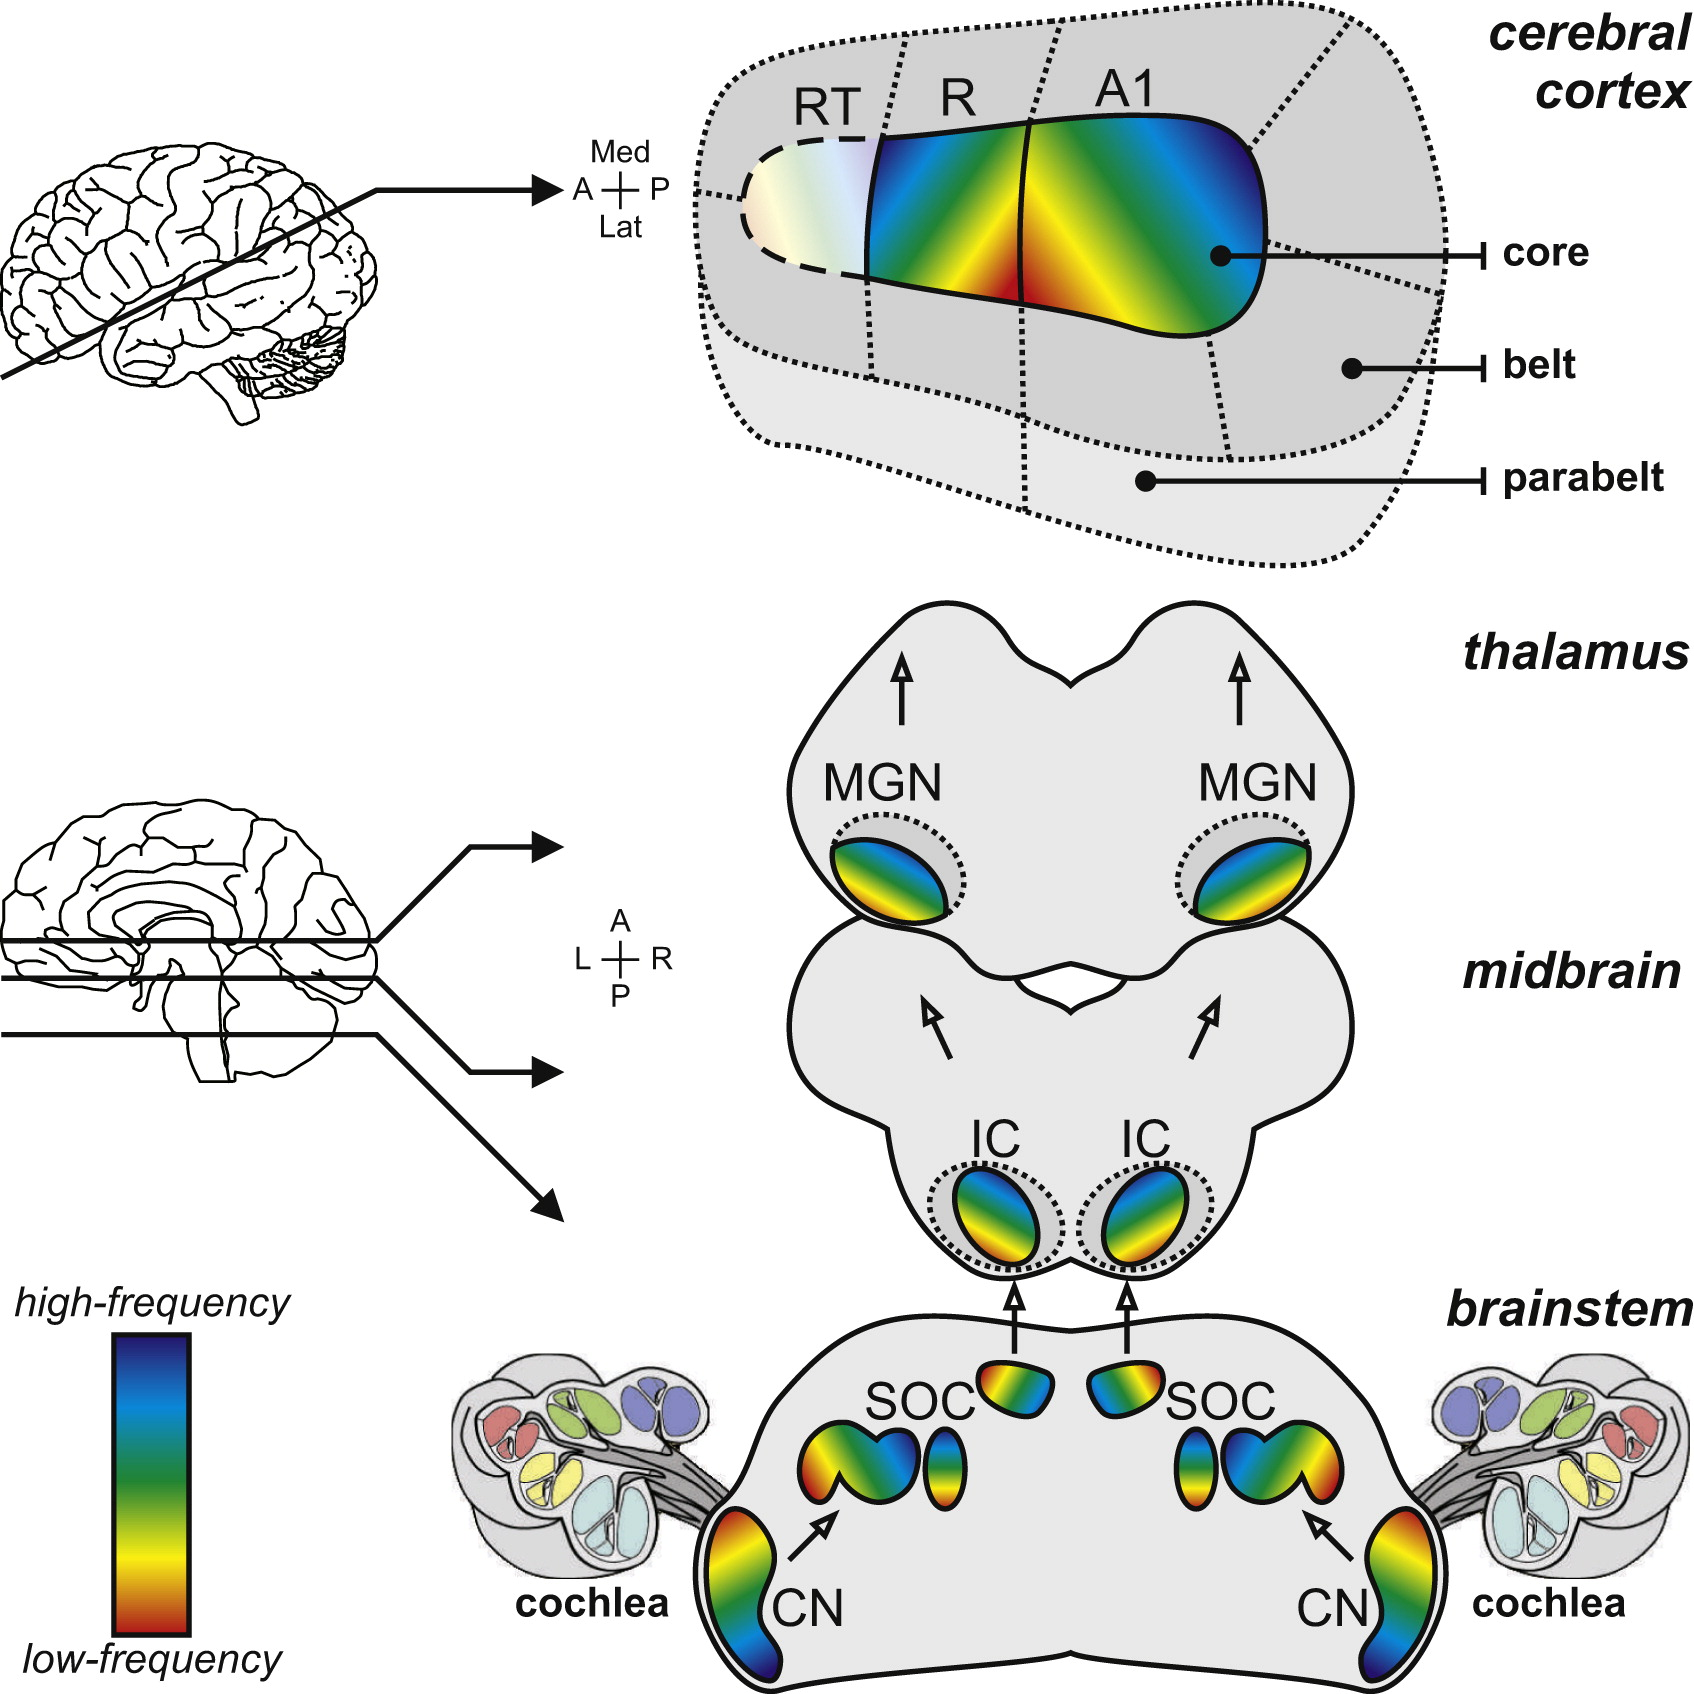
\includegraphics[keepaspectratio]{wk02-2025-01-23_files/mediabag/1-s2.0-S037859551300.jpg}}

}

\caption{{[}Figure 1 from@Saenz2014-ao{]}}

\end{figure}%

\begin{center}\rule{0.5\linewidth}{0.5pt}\end{center}

\begin{figure}[H]

{\centering \pandocbounded{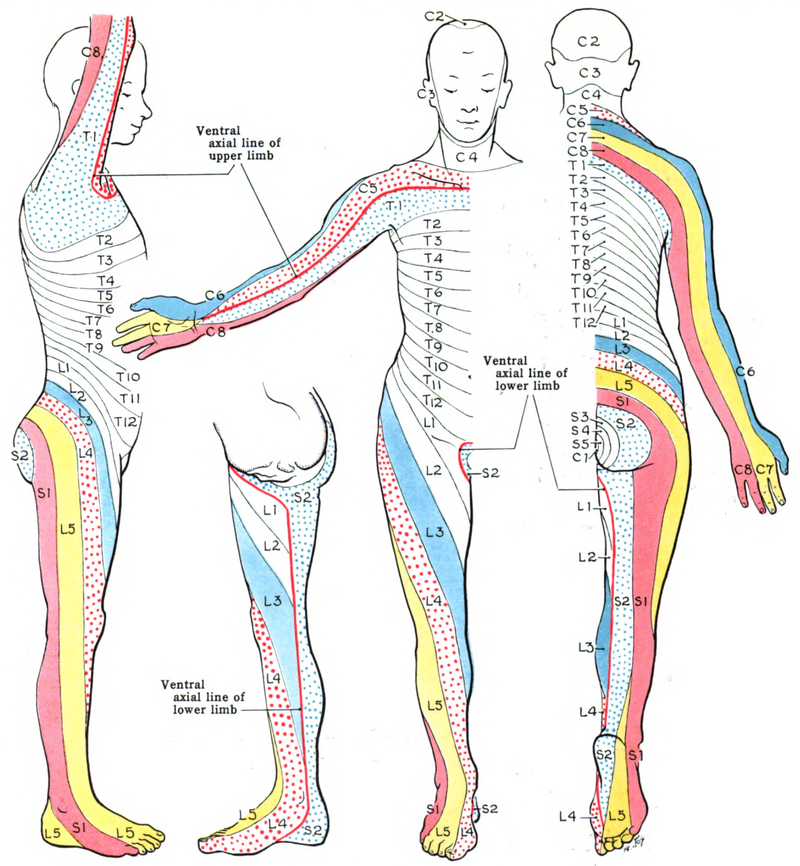
\includegraphics[keepaspectratio]{wk02-2025-01-23_files/mediabag/800px-Grant_1962_663.png}}

}

\caption{Wikipedia}

\end{figure}%

\begin{center}\rule{0.5\linewidth}{0.5pt}\end{center}

\begin{itemize}
\tightlist
\item
  Geometric issues central for perceptual/motor behavior
\item
  Do other systems ``map'' function to structure?
\end{itemize}

\section{Neuroanatomy lab}\label{neuroanatomy-lab}

\subsection{Overview}\label{overview}

\begin{itemize}
\tightlist
\item
  3 groups
\item
  Rotate among stations every \textasciitilde25 min
\item
  Identify as many structures as possible
\end{itemize}

\section{Wrap-up}\label{wrap-up}

\subsection{Main points}\label{main-points}

\begin{itemize}
\tightlist
\item
  Directional terms
\item
  What is it
\item
  Where is it

  \begin{itemize}
  \tightlist
  \item
    Relative to other things
  \item
    CNS/PNS
  \item
    Forebrain/midbrain/hindbrain
  \end{itemize}
\end{itemize}

\begin{center}\rule{0.5\linewidth}{0.5pt}\end{center}

\begin{itemize}
\tightlist
\item
  Cerebral cortex and its subparts
\item
  Grey matter vs.~white matter
\end{itemize}

\subsection{Next time\ldots{}}\label{next-time}

\begin{itemize}
\tightlist
\item
  \href{wk03-2025-01-30.qmd}{Cellular neuroscience I}
\end{itemize}

\section{Resources}\label{resources}

\subsection*{References}\label{references}
\addcontentsline{toc}{subsection}{References}

\phantomsection\label{refs}
\begin{CSLReferences}{1}{0}
\bibitem[\citeproctext]{ref-McNaughton2018-fl}
McNaughton, A. (2018, November 20). Dissecting harriet cole: Uncovering
women's history in the archives. Retrieved January 8, 2025, from
\url{https://drexel.edu/legacy-center/blog/overview/2018/november/dissecting-harriet-cole-uncovering-womens-history-in-the-archives/}

\bibitem[\citeproctext]{ref-swanson2005anatomy}
Swanson, L. W. (2005). Anatomy of the soul as reflected in the cerebral
hemispheres: Neural circuits underlying voluntary control of basic
motivated behaviors. \emph{Journal of Comparative Neurology},
\emph{493}(1), 122--131. \url{https://doi.org/10.1002/cne.20733}

\end{CSLReferences}




\end{document}
